% Copyright James Percent 2013.
% All Rights Reserved.

\documentclass[11pt]{article}
\usepackage{graphics}
\usepackage{amsmath, amsthm, amssymb, latexsym}
\usepackage{hyperref}
\usepackage{draftwatermark}
\begin{document}

\title{\textbf{Unlock: A Framework for Programming Brain-Computer Interfaces}}
\author{James Percent \\
james@shift5.net}
\date{\today}
\parskip 11pt
\parindent 0pt
\maketitle
\tableofcontents
\section{Overview}\label{overviewsec}

Our goal is to develop BCI technology to help individuals suffering from locked-in syndrome~\cite{lis} communicate.  Locked-in syndrome is characterized by an almost complete inability to communicate.  With current technology, unfortunately, we cannot achieve this goal.

We think if more smart people are able to collaborate, then we have a better shot at accomplishing this goal.  Therefore, our strategy is to focus on providing a programming framework that makes it easier for researchers and engineers to build BCI-based systems.  To this end, we employ a few simple ideas.  

We encapsulate as much as possible, which is to say that we separate concerns.  We'll talk more about this later, but the basic idea is that you should not need to know every corner of Unlock to create a new decoding algorithm or add a language model or add a new acquisition device.  

These could be different people with different skill sets, and we want them to be able to dive into their area and be productive quickly.  One of the challenges with BCI technology is that it is inherently cross-disciplinary; therefore, we want to lessen this burden as much as possible.

To support this goal, we need great documentation.  The documentation needs to be encapsulated too.  You should be able to get a high-level idea of how the whole system works and also locate details about your specific area of interest without arduous effort.  

Finally, automate whenever possible; extra batteries included.  We want researchers and engineers to be able to get going quickly.  Learning about all the dependencies and taking a bunch of manual steps can be overwhelming.  Especially if someone just wants to hack out a quick idea.  

In summary, the goal is to give you a great platform to hack out an idea.

The rest of this document is structured as follows.  %In the next section we provide a bit of history.
First we do a quick technical introduction.  After that, we discuss how to install and use Unlock, from a user perspective.  Next, we cover both some of the internals from a high-level.  Finally we close with a example.

Development of the Unlock framework is funded by the Adaptive Brain-Computer Interactions (ABCI) Capstone Project~\cite{abci}.

\section{Technical Introduction}

The infrastructure Unlock provides can be logically separated into two distinct layers: the application layer and the BCI layer.  These layers can in turn be further decomposed.

The BCI layer is defined by the signal-processing chain~\cite{signalprocessing}.  The signal-processing chain includes signal acquisition and reconstruction, feature extraction and decoding, and command generation~\cite{neuraleng}.  Many BCI systems also include a stimulation component, which is actually processed at the application layer; however, logically, the stimulation component is part of the BCI.

For example, a paradigm based on Visually Evoked Potentials (VEP), flashes a graphical sequence at the user, which is subsequently interpreted in the signal-processing chain~\cite{vep}.  But the actual flashing is handled at the application layer.

We'll talk in more detail about the BCI layer in Section~\ref{bcisec}, but for now there is one important take away.  At each point in the pipeline we just discussed, the system is designed so that you can easily decorate, replace or otherwise manipulate the data flow.  Each step in the pipeline is encapsulated under an interface contract.

The application layer is model-view-controller (MVC)~\ref{mvc, mvc1} inspired.  Don't worry too much if you're not familiar with MVC.  It's just a logical framework for structuring graphical user interfaces (GUIs).  

The basic idea is that each application consists of three types of objects: models, views and controllers.  The controllers accept user input (in this case BCI commands) and pass the inputs to the correct models.  Models handle state transformation (the business logic if you will).  Finally, views observe the state objects (models) and render themselves based on the current state of the world.

If you think about it, this also creates a pipeline in the application layer.  The take away here is that these components are also encapsulated under interfaces.

Figure~\ref{bci-pipeline-fig} depicts the main components of Unlock.

%\begin{figure}[]
%\resizebox{\textwidth}{!}{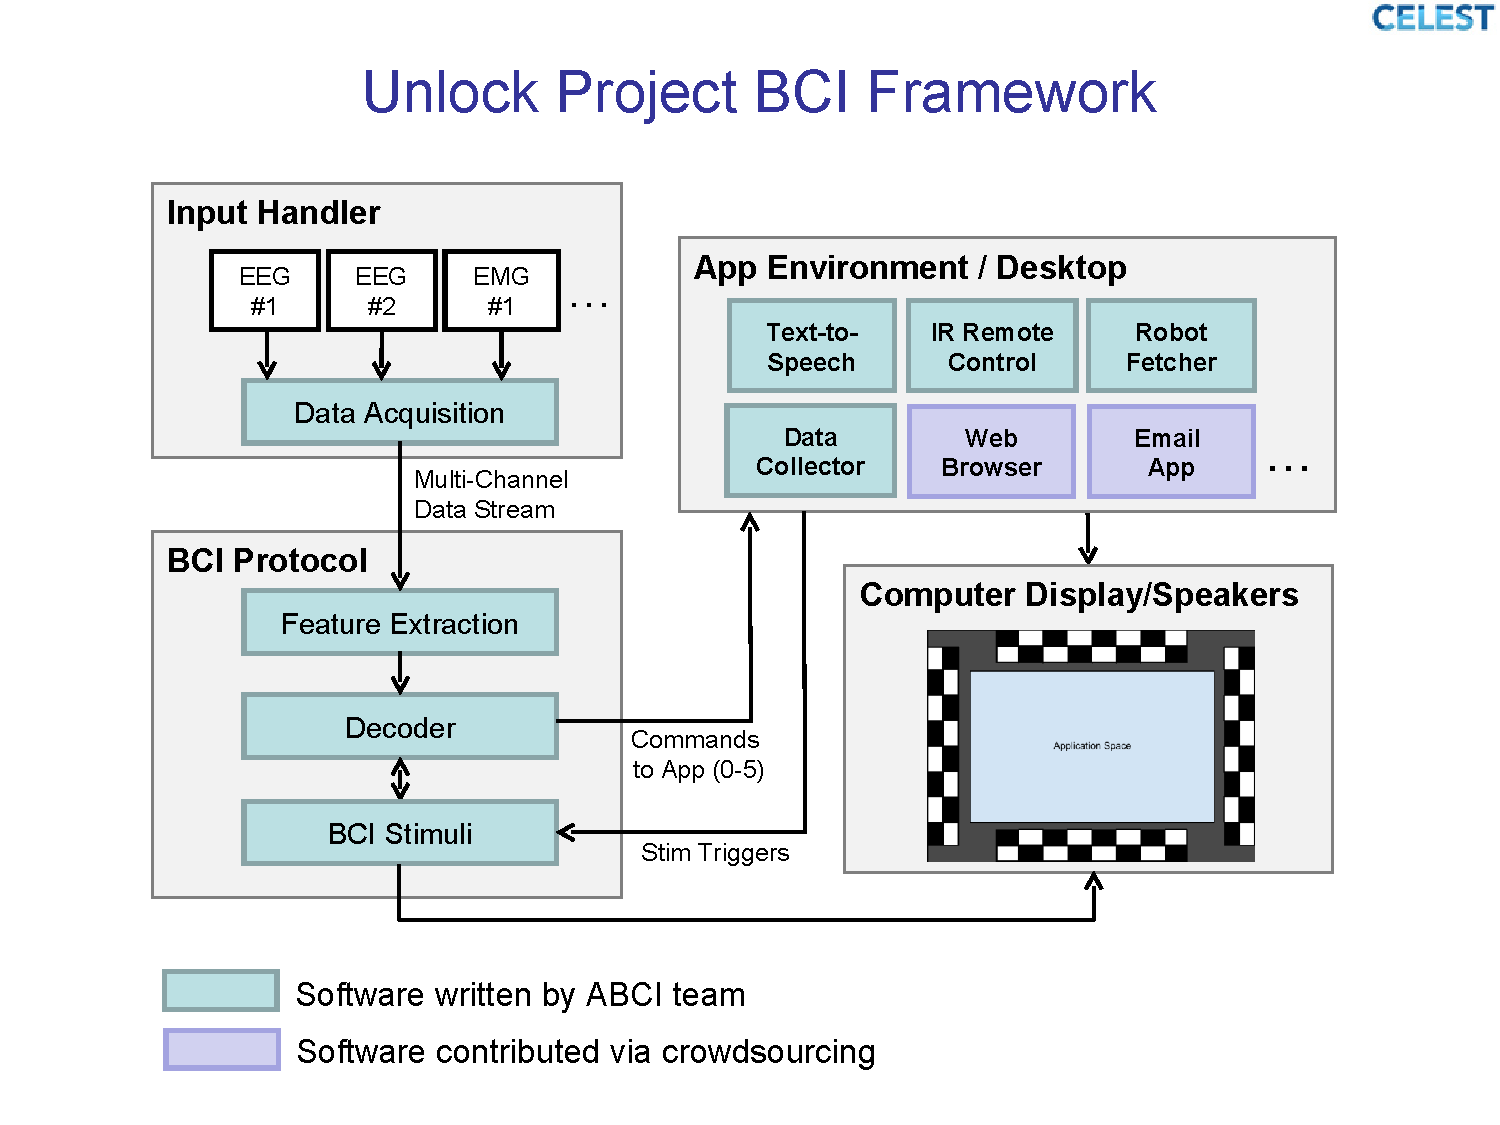
\includegraphics{images/UnlockProjectSoftwareFramework.pdf}}
%\caption{\label{bci-pipeline-fig}  Data flow through Unlock}
%\end{figure}


%\section{History}
%Unlock started, in 2011, as a Python script written by Sean Whatshisname for researching solid-state VEP %(SSVEP)[ssvepref].  In 2012, researching maximium length sequence decoding, Byron Galbraith rewrote Sean's %script into a program.  In 2013, Unlock was completely rewritten to be a programming framework.  The rewrite %was led by James Percent, with help from Byron, Nguyen Hoang Giang and other Unlock contributors. 

\section{Installation}

In the next three sections we describe the installation procedures for Unlock installation on Windows, Linux and Mac OSX.  

\subsection{Windows}

Many signal acquisition devices work exclusively with Windows.  Additionally, many of the potential users of Unlock may only have access to Windows computers.  These circumstances led to Windows being the first platform supported by Unlock.

To make installation on Windows as easy as possible, we decided a binary, click-able installer was the solution that would best suite the community.  There were many ways to proceed, but, ultimately, we decided to write the installer in Go~\cite{golang}.  

The Unlock installer is not much more than a package manager for handling dependencies.  Unlock, not unlike many other frameworks, has many dependencies.  These dependencies include:
\begin{itemize}
\item Avbin10;
\item Flask-0.10;
\item Numpy 1.7.1;
\item Psycopg2 2.5.1;
\item Pyaudio 0.2.7;
\item Pyglet 1.2alpha;
\item Pyserial 2.6;
\item Python 3.3.2;
\item Pywin32 2.1.8;
\item Scikit-learn 0.14.1;
\item Scipy-stack 13.10.11;
\item Scons 2.3.0;
\item SQLAlchemy 0.9.0b1;
\item Visual C++ redistribution 2010.
\end{itemize}

There are additional dependencies based the hardware acquisition device in use.  Unlock supports three acquisition devices.  The National Instruments DAQ, Neural Electronics Enobio, and gtec MOBILab.  

Unfortunately, at the time of this writing, Unlock's C++ layer is built as a single dynamic-link library (dll).  This means all of these dependencies need to be available for Unlock to run.  

Fortunately, Unlock manages all but the NI DAQ driver code.  The NI DAQ dependencies are quasi installed by Unlock, but may require some manual effort.  

The Unlock installer will start the NI DAQ downloader, which should kick off the installer after the download and extraction complete.  But it runs asynchronously to the Unlock installer; the Unlock installer exists without knowing if the NI DAQ installer completed successfully or not; if something happens, go to~\cite{nidaq} and follow the instructions for downloading and installing the NI DAQ.

Most of the dependencies are Python packages.  We played with standard Python packaging systems, such as Pip~\cite{pip} for installing these, but, unfortunately, at the time of this writing, none of these support transitive closure over dependencies.  This makes packaging imperative and error prone.  

Luckily we found~\cite{winpythonpackages}; it has most Python packages as Windows binaries that include their dependencies.  Where ever possible we use the binary package from~\cite{winpythonpackages}.  

We are watching Pip and may revisit using the Pip packages in the future.  That said, Pip would still be wrapped by the Go executable.

\subsubsection{Developer Installation}\label{developerinstallsec}

At this time only developer-based installation is supported.  A developer-based install requires a few steps:
\begin{itemize}
\item install Git Bash;
\item setup a Github account;
\item clone the Github repo;
\item run the binary installer for your architecture (only x86-64 is supported right now).
\item install NI DAQ
\item edit Unlock's config
\item run Unlock to test
\end{itemize}

Go to~\cite{gitbash} for Git Bash download and installation instructions.  

After Git Bash is setup we need to create a Github account~\cite{github} and follow the instructions for setting up an ssh key~\cite{sshkey}.  Next, fork the repo.

After we have your Github account setup we can clone the repo.  This takes a few minutes because we committed all of Unlock's dependencies to the repo.  *Stark* this is generally bad form.  But we are OK with bad form for two related reasons: 1) we are poor and do not have a real server, 2) we care more about keeping everything together more than repo download speed.

To clone the repo run the following command from the Git Bash command.exe:
\begin{verbatim}  
  $ git clone git@github.com:jpercent/unlock.git
\end{verbatim}

Note, git@github.com:jpercent/unlock.git is my fork of the project.  If you want to commit to my fork that's fine, send me email and I'll add you.  But it's probably better to commit to your own fork.  If you want to push changes upstream, then you make a pull request.  

Then change directory to the repo.  To do so type:
\begin{verbatim}
  $ cd unlock/
\end{verbatim}

Then run the installer for a development installation:
\begin{verbatim}
  $ golang/bin/install-win-x86-64.exe -dev=true -repo=`pwd`
\end{verbatim}

Note, the quotes around pwd are back ticks; they tell Bash to execute the command that gets the current working directory.  There should almost immediately be several installers that will ask you questions.  Please accept the defaults on everything.  

Watch the task bar.  Some versions of Windows will bring up access control dialogs; sometimes they come up in the background.  Additionally, at least one of the installers has a dialog that comes up asynchronously and in the background, so keep your eyes peeled for dialog boxes in the background.  They should be flashing on the task bar.

Additionally, AVbin installer puts the avbin.dll in the wrong directory; the installer tries to move it, but you might have to do it manually as the administrator. To fix the issue go to C:\\Windows\\SysWOW64. If there is no avbin.dll, then copy the one in C:\\Windows\\System32 to SysWOW64.

That should be all there is to it.  To test it run the following command:

\begin{verbatim}
  $ export PYTHONPATH=`pwd`
  $ cd unlock/
  $ /c/Python33/python.exe unlock_runtime.py
\end{verbatim} 

If you have an issue, please send me an email directly.  Please include the file named unlock-install.log in the email and a description of the real-time symtom(s).  
 
\subsection{Linux}
\subsection{Mac OSX}
\section{Internals}

\subsection{configuration}
 Unlock builds most components using an "inversion of control" container.  Most people refer to this, nowadays, as dependency injection~\cite{depinjection}.  What it means is that object construction is handled by a container that can be configured to wire up various of configurations based on the contracts/interfaces objects support.  This paradigm of configuration management has been around a long time, but became widely known when the developers of J2EE did not know about it.

The important point, from a mechanical perspective, is that objects rarely create other objects in their own constructors.  In Python each file is referred to as a module.  And each package is defined at the directly level.  Each unlock package has it's own factory that creates objects.  The UnlockFactory creates and wires up the configuration of an unlock instance.  What system is created depends on the values set in the configuration file passed to Unlock.  To understand how dependency injection works let's look at a small example:
\begin{verbatim}
"dashboard" : {
        "main" : true,
        "deps" : {
            "stimulation" : "quad_ssvep",
            "decoder" : "harmonic_sum",
            "controllers" : ["gridspeak", "time_scope", "frequency_scope",
                                  "gridcursor", "fastpad"]
        }
    },
    
    "signal" : {
        "singleton" : 0,
        "name" : "random"
    },

    "window" : {
       "singleton" : 1,
       "name" : "pyglet",
        "args" : {
            "fullscreen" : true,
            "fps" : false,
            "vsync" : false
        }
    },
   
    "harmonic_sum" : {
        "deps" : {
            "buffering_decoder" : "fixed_time_buffering_decoder",
            "threshold_decoder" : "absolute_threshold_decoder"
        },
        
        "args" : {
           "fs" : 256,
           "trial_length" : 3,
           "n_electrodes" : 8,
           "targets" : [12.0, 13.0, 14.0, 15.0],
           "target_window" : 0.1,
           "nfft" : 2048,
           "n_harmonics" : 1
        }
    }
\end{verbatim}

There are 4 elements here: "dashboard",  "signal", "window" and "harmonic\_sum".  Here we are using JSON as the configuration language. 

Each object that has an attribute named "singleton" is created automatically by the UnlockFactory and is available to any of the other objects listed in the config file by it's name.  Note that the name is not the "name" attribute; the "name" attribute is actually the type, which it probably should be changed to.  The order they are created in depends on the value of the "singleton" attribute - this allow us to support a dependency hierarchy.  For example, the "window" singleton, which is of type pyglet\_window, must be created after the "signal" singleton, which is of type random.  I may remove this dependency hierarchy in favor of transitive closure over dependencies, but this was more simple to get started.  For singletons a name attribute must be supplied; it corresponds directly with an UnlockFactory method - i.e. there is an unlock factory method named random, and 1 named pyglet\_window.

Objects with the "singleton" attribute are created later.   Note that the "dashboard" object has "main" set to true.  This is the only none singleton object that will be created independently.  Everyother object that gets created, must have a dependency off of the main object.  For example, the "dashboard" lists "harmonic\_sum" inside its "deps" json object.  Primitive arguments are passed to a factory method using the "args" json object and complex objects are passed using the "deps".  I may merge these together and make the factory a bit smarter, but this was simpler to start and that's how I learned to program (make it simple, make it work, then optimize).

\subsection{BCI Layer}\label{bcisec}

In Section~\ref{overviewsec} we defined the signal-processing chain to be signal acquisition and reconstruction, feature extraction and decoding, and command generation.

\subsubsection{Stimulation}

\subsubsection{Acquisition}\label{acquisitionsec}

Most of the signal acquisition code is written in C++.  The C++ layer is dynamically linked to the Python run-time using Boost Python~\cite{boostpython}.  The C++ signal acquisition module exports a single polymorphic interface inspired by UNIX device files, and several factory methods for creating the signal acquisition infrastructure.

Unlock supports two modes of acquisition: blocking acquisition and non-blocking acquisition.  Blocking acquisition is is simply a thin wrapper around the device interface.  It will block on a I/O descriptor until a write is available.

We will discuss Unlock's application layer in detail in Section~\ref{applicationsec}.  But at this time it is important to understand one aspect.  The application layer is essentially a graphics event loop; looping through the application layer code at each screen refresh.  To acquire the signal on the same thread as the graphics event loop is problematic: blocking on each screen refresh can cause all kinds of problems.  In fact, blocking-based acquisition is only supported for device testing purposes. 

To acquire the signal without blocking, Unlock supports a non-blocking acquisition mode.  In non-blocking mode, Unlock creates a platform independent C++ thread that manages and buffers the signal data.  The graphics event loop synchronizes with the signal acquisition thread using a lock-free algorithm.  The method makes use of a ring buffer and processor level atomic instructions to coherently reserve blocks of virtual memory addresses across cores.

\subsubsection{Decoding}

\subsubsection{Command Generation}

\subsection{Application Layer}\label{applicationsec}

The Unlock application programming layer is a model-view-controller (MVC)~\cite{mvc, mvc2} inspired framework for graphical user interface (GUI) development.  Commands flow through the BCI layer to a control layer that interprets the state changes and sends the changes to visualization module.

\subsection{Compiling Unlock's C++ code}

The acquisition software, described in~\ref{acquisitionsec}, includes C++ software that interfaces with data acquisition devices and links with the Python runtime.  This section describes how to compile the C++ software.  This section assumes the developer installation instructions~\ref{developerinstallsec} have been completed.  

Scons-2.3.0~\cite{scons}, a Python-based, cross-platform build system, is the system used to build Unlock's C++ software.  The Scons documentation can be found here~\cite{sconsdocs}.  Scons requires Python27, so you must install Python27 to build Unlock's C++ software.

The C++ is located under \textit{unlock/bci/acquire-c++}.   In \textit{acquire-c++}, \textit{build.py} automates the enviornment setup and build process and installation of binaries.

\begin{verbatim}
	jpercent@feynman ~/unlock/unlock/bci/acquire-c++ (master)
	$ /c/Python33/python.exe build.py --help
	Usage: build.py [options]

	Options:
  	--version             show program's version number and exit
  	-h, --help            show this help message and exit
  	-n, --runtime-dir  sets the installation directory; defaults to ..cquire
  	-p, --python         specifies the location of the python interpreter; default
        	                  is c:\Python27\python.exe
        -o, --scons          specifies the location of the scons script; default is
                                 c:\Python27\Scripts\scons-2.3.0.py
        -l, --lib-dir          sets the library directory to copy binaries to; default
                                 is lib\win-x86-msvc-10, relative the build directory
        -c, --clean          removes old binaries before building
        -s, --setup         configures the build environment for the first time; must
                                be run with the first build
        -i, --install         configures the build environment for the first time; must
                                be run with the first build
        -b, --build          builds the libraries and tests and copies them to the
                                library directory
\end{verbatim}

The very first time \textit{build.py} is executed, the \textit{-s} option must be included.  It can be run as follows.
\begin{verbatim}
    $ /c/Python33/python.exe build.py --setup
    $  /c/Python33/python.exe build.py --clean --build --install

                    or

    $ /c/Python33/python.exe build.py -s -c -b -i
\end{verbatim}

The build will fail if the setup is not executed.  If the script works, then the packages are built and installed, and the world is a happy place.  

In the rest of this section, the manual steps of building are explained; if \textit{build.py} fails, we do not want to leave anyone stuck.

The setup option, untars the C++ include files required, installs Python27 and installs Scons-2.3.0 into the Python27 distribution.  These steps can be accomplished by running the following commands from Git Bash.  Note that we are in the \textit{acquire-c++} directory.

\begin{verbatim}
    $ tar xzvf includes.tar.gz  && cmd.exe "/C install-python27.bat"  && \ 
       cd ../../../package  && tar xzvf scons-2.3.0.tar.gz && \
       cd scons-2.3.0 && /c/Python27/python.exe install setup.py  
\end{verbatim}

To build the source run Scons with the \textit{\-Q} option. We recommend cleaning the old binaries before compiling; to do so run Scons with the \textit{\-c} option.  An example follows.
\begin{verbatim}
    $ /c/Python27/python.exe /c/Python27/Scripts/scons-2.3.0.py -c 
    $ /c/Python27/python.exe /c/Python27/Scripts/scons-2.3.0.py -Q
\end{verbatim}

If the build completes successfully, then a number of libraries and executables will be created and placed into a platform specific subdirectory of \textit{acquire-c++/lib/}.  The final steps involve installing the binaries we just built.  The installation steps are platform independent and covered in the next 3 sections.

\subsubsection{Windows x86-64}

On Windows, the platform specific subdirectory is named \textit{acquire-c++/lib/win-x86-msvc-10}.  Note, on Windows x86-64, the Unlock C++ code is actually x86.  The final step is to put the files into a place where the python interpreter can find them at runtime.

In a Windows environment, there is no notion of a dynamic link library search path, so dependencies that are not in the system directory need to be in the same working directory when loaded.  This means we need to co-locate our library with all of its non-system dependencies.

The following command, run from the bci directory, will copy our libraries and their dependencies.

\begin{verbatim}
    $ cp acquire\-c++/lib/win-x86-msvc-10/*.dll acquire-c++/*exe acquire/
\end{verbatim}

Next we need to rename \textit{neuralsignal\_win\_x86.dll}; this file is a binary Python module and the python interpreter will not load .dll files when it loads the acquire package.  It will only load .pyd files.  We also need to remove the platform dependency on the name.  The following command, run from the acquire directory, will accomplish this.

\begin{verbatim}
    $ cp neuralsignal_win_x86.dll neuralsignal.pyd
\end{verbatim}

Note, that we do not rename the file but make a copy of it.  This is because the tests use the names of the original binaries and we want to be able to run the tests as a sanity check.

\subsubsection{Linux}
\subsubsection{Darwin}

\begin{thebibliography}{99}
\bibitem{lis}  Bauer, G. and Gerstenbrand, F. and Rumpl, E. Varieties of the locked-in syndrome. Journal of Neurology.  1979.
\bibitem{signalprocessing}  Sippi, C.,  Sippi, P., Computer Dictionary and Handbook. 1972. 
\bibitem{neuraleng}  He B., Gao S., Yuan H., and Wolpaw, J.  Neural Engineering, Chapter 2, Brain–Computer Interfaces.  2013.
\bibitem{abci} CELEST Capstone Project 1: Adaptive Brain-Computer Interactions.  http://celest.bu.edu/about-us/capstone-projects/adaptive-brain-computer-interactions.
\bibitem{mvc}  Reenskaug, T. A note on DynaBook requirements. Xerox PARC.  1979.
\bibitem{vep} O’Shea, R. P., Roeber, U., Bach, M. Evoked potentials: Vision.  Encyclopedia of Perception. 2010.
\bibitem{boostpython} Boost Python.  http://www.boost.org/doc/libs/1\_54\_0/libs/python/doc/.
\bibitem {npl} Unlock.  http://github.com/jpercent/unlock.
\bibitem{golang} Go.  http://golang.org.
\bibitem{winpythonpackages}  Christoph Gohlke.  http://www.lfd.uci.edu/~gohlke/pythonlibs/.  Laboratory for Fluorescence Dynamics, University of California, Irvine.
\bibitem{pip} PIP.  https://github.com/pypa/pip.
\bibitem{nidaq} NI DAQ.  http://www.ni.com/dataacquisition/nidaqmx.htm.
\bibitem{pubsub} Eugster, P.  Felber, P.  Guerraoui, R.  Anne-Marie Kermarrec, A.  The many faces of publish/subscribe.  ACM Computing Surveys (CSUR) Surveys Homepage table of contents archive.  2003.
\bibitem{mobilab} Gtec MOBILab.  http://www.gtec.at/Products/Hardware-and-Accessories/g.MOBIlab-Specs-Features
\bibitem{gitbash} Git Bash.  http://git-scm.com/download/win.
\bibitem{depinjection} Fowler, M.  Fowler, Martin.  Inversion of Control Containers and the Dependency Injection pattern.  http://martinfowler.com/articles/injection.html.  2003.  
\bibitem{scons}  Scons.  http://www.scons.org/.
\bibitem{sconsdocs} Scons 2.3.0 User Guide.  http://www.scons.org/doc/2.3.0/HTML/scons-user/.
\bibitem{observer} Observer pattern.  https://en.wikipedia.org/wiki/Observer\_pattern
\bibitem{github}  Github.  https://github.com.
\bibitem{sshkey} Github SSH key Generation.  https://help.github.com/articles/generating-ssh-keys.
\end{thebibliography}

\end{document}
